\chapter{Proposed Methodology}
\label{chap3}
In the previous chapter, we have discussed the theories that support this research related to the Electronic Voting Machine . In this chapter we will proposed our methodology for this project.
\section{Block Diagram}
Let us look at the simplified block diagram in Figure \ref{blockDiagram}, which illustrates the main components involved
in Electronic Voting Machine(EVM) Using 8051 Micro-controller. Switches are used to make choices, resister, capacitor, and oscillator are being used to work the micro-controller properly on the circuits with the help of connecting wires.
\begin{figure}[H]  %h=positioning
\begin{center}
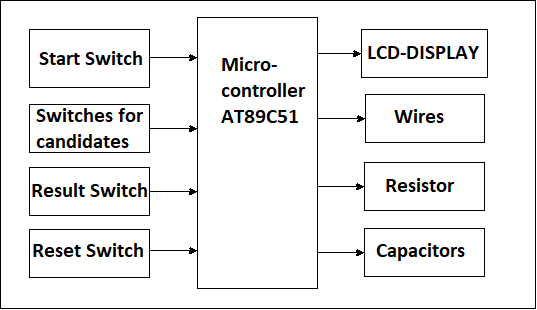
\includegraphics[scale=0.80]{Chapter3/blockDiagram}
\caption{Simplified Block Diagram of Electronic Voting Machine(EVM) Using 8051 Microcontroller}
\label{blockDiagram}
\end{center}
\end{figure}


\section{Components Selection}
\subsection{Hardware Components}
Following is the components which we have used to implement Electronic Voting Machine(EVM) Using 8051 Microcontroller.
\begin{figure}[H]  %h=positioning
\begin{center}
\includegraphics[scale=0.95]{Chapter3/comp1}
%\caption{Simplified Block Diagram of Electronic Voting Machine(EVM) Using 8051 Microcontroller}
%\label{blockDiagram}
\end{center}
\end{figure}
\begin{figure}[H]  %h=positioning
\begin{center}
\includegraphics[scale=0.95]{Chapter3/comp2}
%\caption{Simplified Block Diagram of Electronic Voting Machine(EVM) Using 8051 Microcontroller}
%\label{blockDiagram}
\end{center}
\end{figure}


\subsection{Software Selection}
To simulate our project, we have used proteus, the Proteus Design Suite is a proprietary software tool suite used primarily for electronic design automation. The software is used mainly by electronic design engineers and technicians to create schematics and electronic prints for manufacturing printed circuit boards. \begin{figure}[H]  %h=positioning
\begin{center}
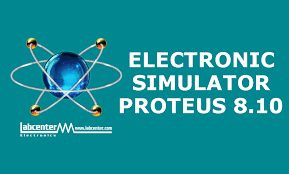
\includegraphics[scale= 1.5]{Chapter3/proteus}
%\caption{Simplified Block Diagram of Electronic Voting Machine(EVM) Using 8051 Microcontroller}
%\label{blockDiagram}
\end{center}
\end{figure}
